\workpkg{1}

%% This Work Package deals with the mission functional analysis, the
%% definition of the spacecraft requirements and the mission profile,
%% and the initial sizing of your spacecraft.

%% WP1.1 Functional Analysis
%% WP1.2 Spacecraft Requirements
%% WP1.3 Mission Profile
%% WP1.4 Initial Sizing

%% Timeline : Weeks 1 and 2 (2-weeks total duration)

%% Deadline for Report Delivery: Monday September 17th, 12.00 hours

%% Each report shall include, as a minimum, all the Deliverables
%% listed in the sub-WP descriptions provided below (each deliverable
%% is identified by a unique code, in the form Dx.y.z). The names and
%% student numbers of the authors shall be present on the cover
%% page. The report shall also include a work division table,
%% indicating which group members have contributed to each one of the
%% tasks.

%% Deliver the printed report to the Teaching Assistant assigned to
%% your group.

\subworkpkg{1.1}

%% Tasks

%% A. Search for 5 existing (or planned) similar missions and identify
%% for these missions:

%% a. the mission objectives and, if possible, the associated mission
%% requirements;

%% b. the main elements that make up the mission and their main
%% function(s);

%% c. the main performance and design characteristics of these
%% elements.

%% B. Define the mission elements with which the design process will
%% interact (e.g.: mission operations, ground system, launch system,
%% etc.).

%% C. List the main objectives to be achieved in the design process
%% (related to, e.g., payload capability, performance, structure,
%% etc.). Mention at least 10 objectives.

%% D. For each one of the identified design objectives, list the main
%% functionalities that the design must provide in order to accomplish
%% it.

%% E. List all the design parameters that are already available (e.g.,
%% from the project description provided in Section 3) and the ones
%% which still need to be identified.

%% Deliverables

%% D1.1.1. Comparative table including all the relevant information
%% collected for the reference missions identified under Task A above.

\deliverable{1.1.1}

%% D1.1.2. Block diagram showing the outcomes of Task B above (hint:
%% you can put the item to be designed in the middle, and the relevant
%% mission elements around it).

\task{B}

The design will have to interact with the following mission elements.

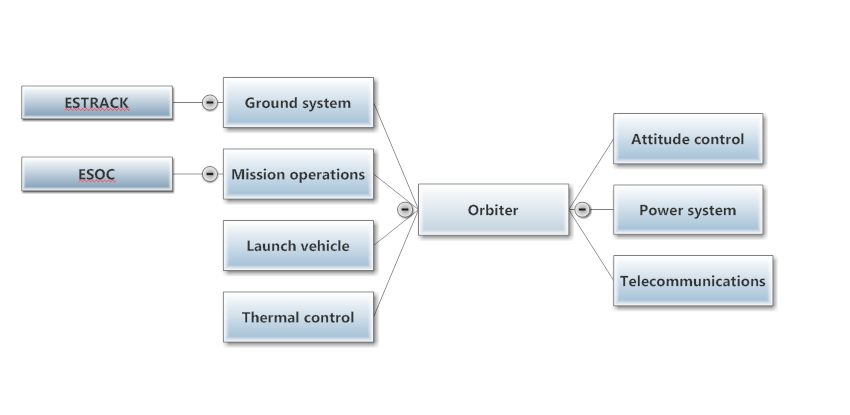
\includegraphics[width=\textwidth]{block-diagram-WP1-1B}

\begin{itemize}
\item{Ground system.} The ground segment will use ESTRACK.
\item{Mission operations.} The mission operations center will be ESOC.
\item{Launch vehicle.}
\item{Thermal control.}
\item{Attitude control.}
\item{Power system.}
\item{Telecommunications.}
\item{Radiation shielding.}
\item{Propulsion systems.}
\item{S/C structures.}
\item{Orbit / trajectory}
\end{itemize}

\deliverable{1.1.2}

%% D1.1.3. Numbered lists obtained from Tasks C, D and E above (note:
%% lists should be as complete as it is possible at this stage of the
%% design, and a clear justification for each listed item shall be
%% provided).

\task{E}

The already known design parameters are

\begin{enumerate}
\item{Payload mass.} 80kg
\item{Payload dimensions.} 0.7m x 0.7m x 0.7m
\item{Payload required power.} 50W
\item{Payload operational temperature range.} 150--200K
\item{Orbit.} Polar, 200km above Europa surface.
\item{Mission duration.} At least 3 years in Europa orbit.
\item{Launch date.} 2020
\item{Total mission cost.} Less than 500 million FY2000 USD.
\item{Mission reliability.} 0.9
\end{enumerate}

The design parameters yet to be determined include

\begin{enumerate}
\item{Radiation environment.} Radiations levels demand adequate
  shielding.
\end{enumerate}

\deliverable{1.1.3}

\subworkpkg{1.2}

%% Tasks

%% A. Familiarize with the celestial body object of the mission (Moon,
%% Mars or Europa) and collect all the relevant information on it
%% (e.g., gravitation coefficient, radius, atmospheric density,
%% orbital period, eclipse periods, solar intensity received, albedo,
%% etc.).

%% B. Search for at least 5 existing (or planned) spacecrafts to be
%% used as a reference for your design, i.e.  for which the S/C
%% specifications and characteristics are similar to the ones expected
%% in your mission.  Collect information on the design of the
%% identified reference spacecrafts (e.g., mass and power budgets,
%% size, structure configuration, payload characteristics, orbital
%% parameters, etc.).

%% C. List a detailed set of requirements for your design, taking into
%% account the top-level mission requirements (from the project
%% description provided in Section 3) and the characteristics of the
%% identified reference spacecrafts. Remember: the requirements shall
%% be SMART (Specific, Measurable, Achievable, Realistic,
%% Time-bound)!! Whereas possible express them as numbers, preferably
%% in the form of a range of values.

%% D. From the complete list of requirements, identify at least 10
%% driving requirements for your design, i.e.  requirements that will
%% play a major role in the design process. Provide an adequate
%% justification for your choice.

%% Deliverables

%% D1.2.1. Table including all the relevant data on the celestial body
%% object of the mission.

\deliverable{1.2.1}

Data is from \cite{nasaeuropa} and other sources which should be added.

\begin{itemize}
\item{Orbit Size Around Jupiter (semi-major axis):}  671,100 km
\item{Periapsis (closest):}  664,792 km
\item{Apoapsis (farthest):}  677,408 km
\item{Sidereal Orbit Period (Length of Year):} 3.551181041 Earth days
\item{Orbit Circumference:}  4,216,552.51 km
\item{Average Orbit Velocity:}  49,476.1 km/h
\item{Orbit Eccentricity:} 0.0094
\item{Orbit Inclination:} 0.466 degree
\item{Mean Radius:}  1,560.8 km
\item{Equatorial Circumference:}  9806.8 km
\item{Volume:}  15,926,867,918 \si{km^3}
\item{Mass:}  47,998,438,387,492,700,000,000 kg
\item{Planet density:}  3.013 \si{g/cm^3}
\item{Surface Area:}  30,612,893.23 \si{km^2}
\item{Surface Gravity:}  1.315 \si{m/s^2}
\item{Escape Velocity:}  7,293 km/h. Scientific Notation: 2026 m/s
\item{Sidereal Rotation Period (Length of Day):} 3.551 Earth days
\item{Atmospheric Constituents:} Oxygen
\item{Temperature:} 102K
\item{Albedo:} 0.67
\item{Solar intensity:} 49.8 \si{W/m^2}
\end{itemize}

%% D1.2.2. Comparative table including all the relevant design data
%% collected for the reference spacecrafts identified under Task B
%% above.

\deliverable{1.2.2}

%% D1.2.3. Detailed list of design requirements, with a clear
%% indication of the driving requirements.

\deliverable{1.2.3}

\subworkpkg{1.3}

%% Tasks

%% A. Using methods based on statistical data (like, for instance, the
%% ones presented in Ref. [1]), make a first vehicle level estimation
%% of the spacecraft dry mass, power, size, reliability and
%% cost. Hint: you can use the reference spacecrafts characteristics
%% found in the framework of WP 1.2 to evaluate the accuracy of the
%% methods you have adopted, or even to develop your own estimation
%% method.

%% B. Preliminarily define the orbital parameters (a, e, i, , ) and
%% the interplanetary transfer trajectory foreseen for your mission.

%% C. Estimate the total v required by the mission and, based on
%% this, the total propellant mass needed (note: this value depends on
%% the type of engines/thrusters you use!! If this has not been
%% decided yet in detail, you may still have several open options for
%% the propellant mass at this stage…). Include in your estimation all
%% the relevant mission phases (e.g. launch, transfer, orbit
%% corrections, station keeping, interplanetary transfer, etc.). Don’t
%% forget to take into account proper margins!! Hint: you can use the
%% data referred to similar missions, found in the framework of WP
%% 1.1, as a baseline for your estimation.

%% D. Choose an adequate launcher for your mission and, consequently,
%% indicate the launch location, sketch the ascent profile, estimate
%% the maximum launch loads and the required minimum longitudinal and
%% transversal natural frequencies, and identify the payload adapters
%% available for use and their characteristics.

%% E. Based on the information obtained from the previous Tasks,
%% generate a detailed mission profile and a rough timeline for the
%% mission.

%% Deliverables

%% D1.3.1. Vehicle-level estimation of the spacecraft dry mass,
%% propellant mass, power, size, reliability and cost.

\deliverable{1.3.1}

%% D1.3.2. Complete mission profile (including a description of the
%% launcher requirements and characteristics) and preliminary mission
%% timeline up to EOL (End Of Life).

\deliverable{1.3.2}

%% D1.3.3. Graphical sketch of the spacecraft trajectory during all
%% the phases of the mission, including launch, ascent, separation,
%% parking orbit(s), interplanetary transfer and final orbit.

\deliverable{1.3.3}

%% D1.3.4. Table showing the orbital parameters characterizing the
%% spacecraft final orbit.

\deliverable{1.3.4}

%% D1.3.5. Estimated total v required by the mission, including a
%% table showing its breakdown into all the contributions related to
%% different mission phases and operations.

\deliverable{1.3.5}

\subworkpkg{1.4}

%% Tasks

%% A. Using methods based on statistical data and/or empirical
%% relationships (like, for instance, the ones presented in Refs. [1]
%% and [2]), define the preliminary mass and power budgets for the
%% spacecraft, i.e.  the mass and power distribution among all the
%% relevant subsystems. Pay particular attention to the definition of
%% proper design margins in your budgets.

%% B. Based on the information gathered so far, roughly sketch at
%% least three different preliminary architectures of the spacecraft
%% with its main components (e.g. antennae, solar arrays, batteries,
%% nuclear generator, payload units, external skin). Draft at least
%% one of these preliminary sketches as a CATIA drawing.

%% C. For each one of the proposed preliminary architectures, estimate
%% the vehicle MMOI (Mass Moment of Inertia) both for the deployed and
%% un-deployed state.  Deliverables

%% D1.4.1. Tables showing the preliminary mass and power budgets for
%% the spacecraft.

\deliverable{1.4.1}

%% D1.4.2. Sketches of different optional preliminary spacecraft
%% architectures.

\deliverable{1.4.2}

%% D1.4.3. CATIA drawing of at least one preliminary spacecraft
%% architecture.

\deliverable{1.4.3}

%% D1.4.4. Estimation of the vehicle MMOI in the deployed and
%% un-deployed state.

\deliverable{1.4.4}
